\section{Experiment 3 : Improve Relevance Propagation}
The results from the previous experiment show that better structured cell architecture leads to better explanation, in other words, easier to be explained. However, there are some cases that the purposed architectures fail to distribute relevance properly.  Hence, this experiment aims to extend the proposed architectures further to better address the problem. More precisely, we consider the same setting as Section \ref{sec:exp2_prob_formulate}. Here, we propose 3 improvements, namely stationary dropout, employing gating units,  and literal connections of convolutional layers.


\subsection{Proposal 1 :  Stationary Dropout}
Dropout is a simple regularization technique that randomly suspends activity of neurons during training\cite{SrivastavaDropoutSimpleWay2014} . This randomized suspension allows the neurons to learn more specific representations and reduces chance of overfitting.  As a result, its influence directly impacts the quality of explanation. 

%\addfigure{\ref{fig:lenet_various_dropout}} shows explanations of LeNet trained with different dropout probability.

%\begin{figure}[!htb]
%\centering
%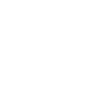
\includegraphics[draft,width=0.5\textwidth]{/sketch/placeholder}
%\caption{LeNet with various dropout values} 
%\label{fig:lenet_various_dropout}  
%\end{figure}



\begin{figure}[!htb]
\centering
\subfloat[Naive Dropout]{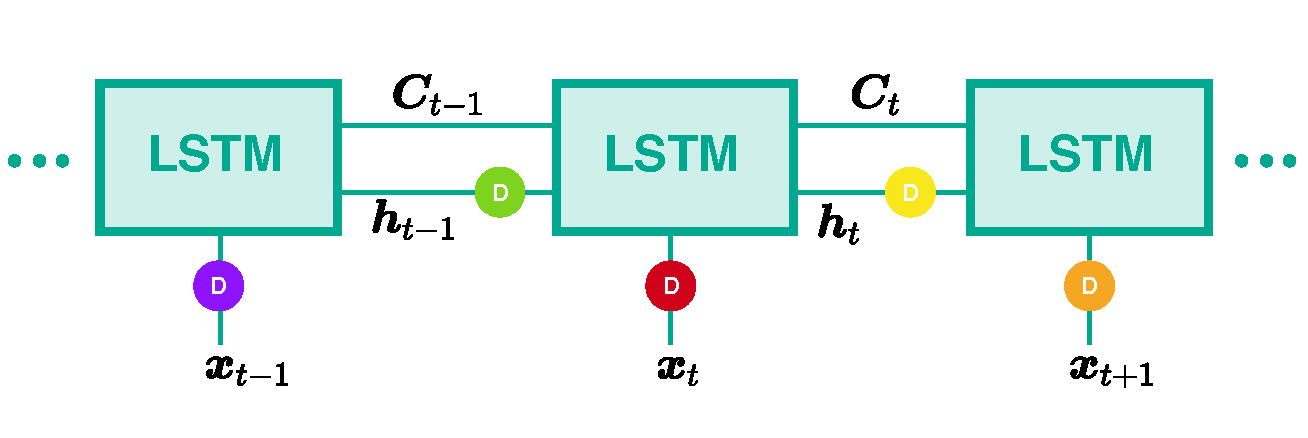
\includegraphics[width=0.8\textwidth]{sketch/lstm_naive_dropout} \label{fig:lstm_naive_dropout}} \\
\subfloat[Stationary Dropout]{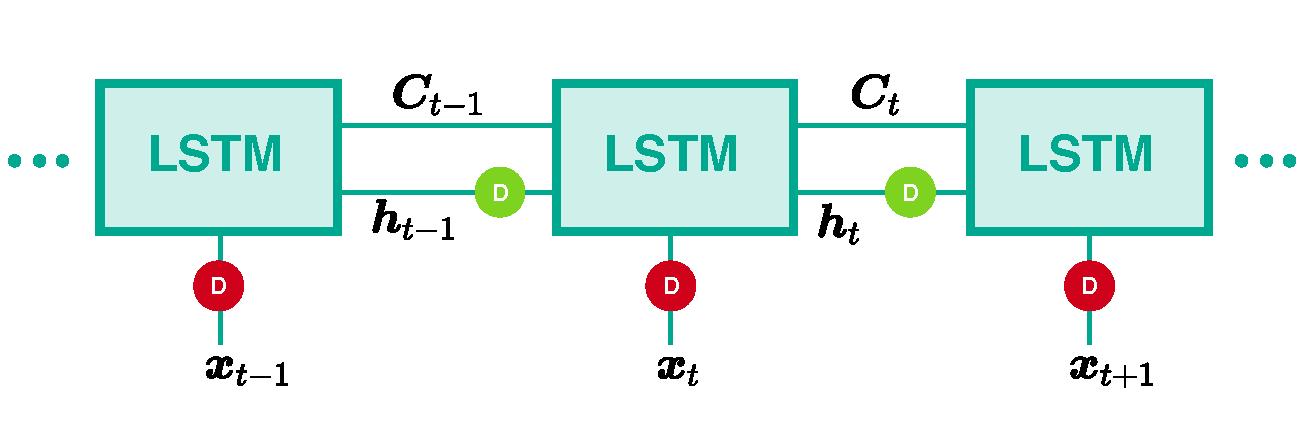
\includegraphics[width=0.8\textwidth]{sketch/lstm_variational_dropout} \label{fig:lstm_variational_dropout}}

\patcaption{LSTM with different dropout approaches.}{\textcircled{\tiny \textbf D} indicates a dropout mask and its color represents the suspension activity.}
\label{fig:dropout_lstm}
\end{figure}

However, unlike typical feedforward architectures, RNN layers are reused across time step, hence a question arises whether the same neurons in those layers should be suspended or they should be different neurons when applying the layers multiple times. \addfigure{\ref{fig:dropout_lstm}} illustrates these 2 different approaches where different colors represent different dropping activities. In particular, this stationary dropout was first proposed by \cite{GalTheoreticallyGroundedApplication2016} who applied  the technique to LSTM and GRU and found accuracy improvements on language modeling tasks.

\subsection{Proposal 2 : Gating units}
\begin{figure}[!htb]
\centering
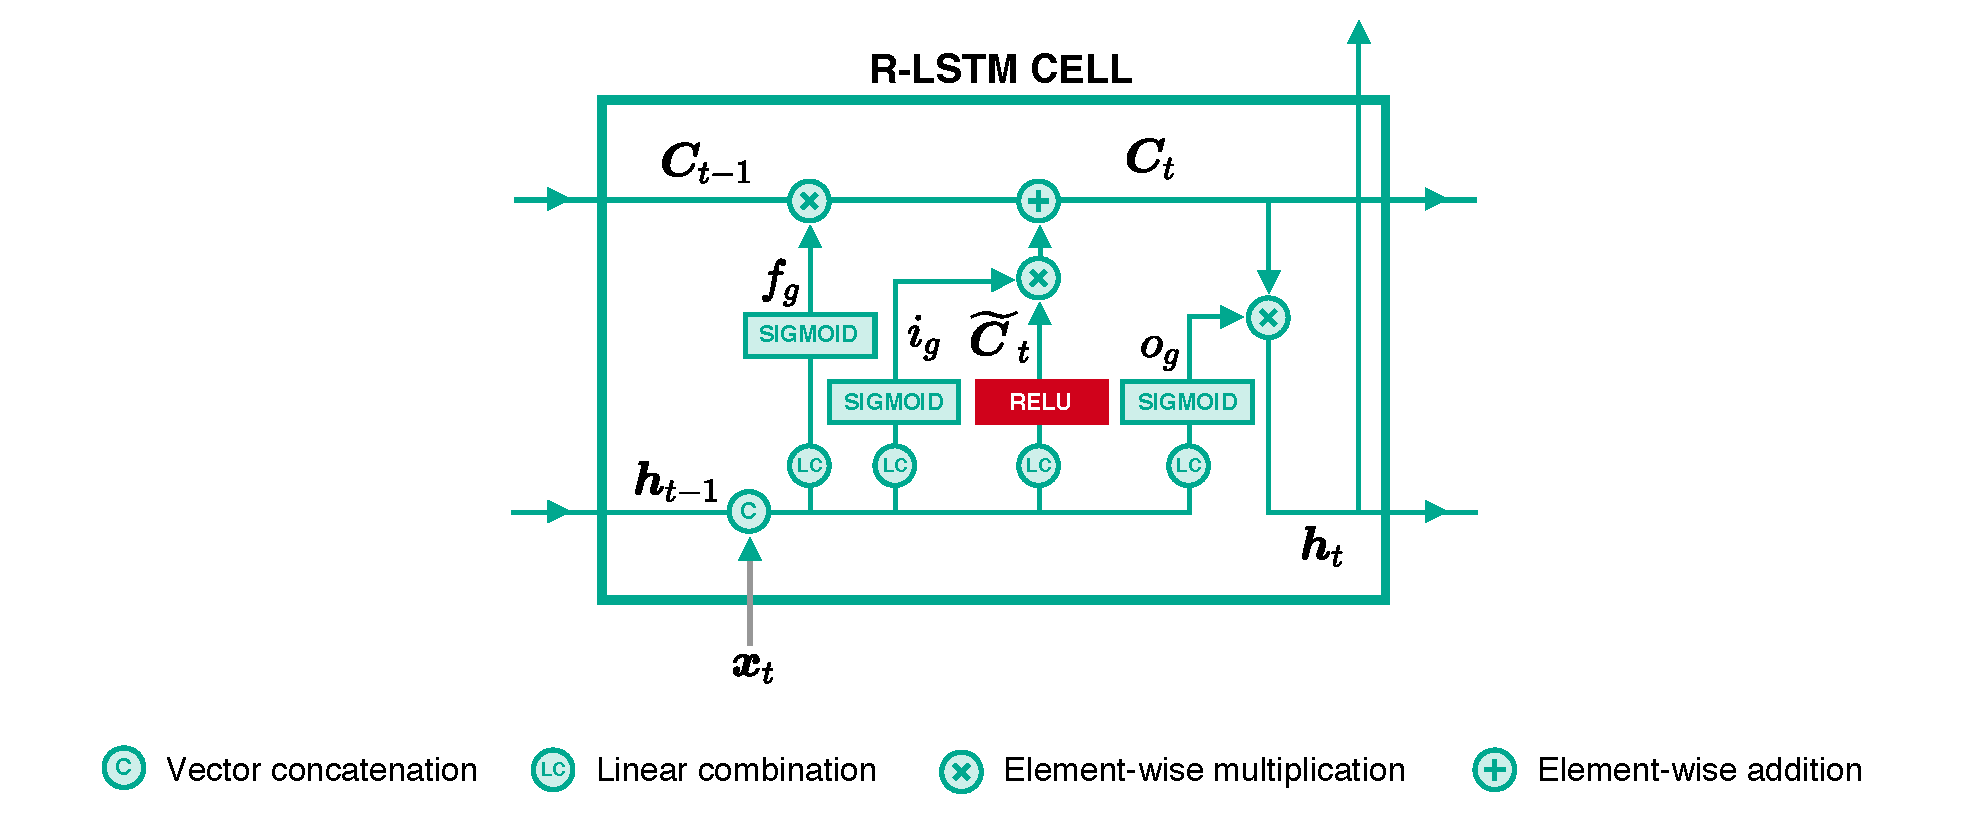
\includegraphics[width=1\textwidth]{sketch/relu_lstm}
\caption{R-LSTM Structure} 

\label{fig:relu_lstm} 
\end{figure}

It is already shown that gating units and addictive updates are critical mechanisms that enable LSTM to learn long term dependencies \cite{GreffLSTMsearchspace2017, Jozefowiczempiricalexplorationrecurrent2015a}. However, LSTM is not readily applicable for methods we are considering in this thesis. More precisely, the use of sigmoid and tanh activations violates the assumption of GB and DTD. Therefore, we propose a slight modified version of LSTM where ReLU activations are used to compute cell state candidates $\widetilde{C}_t$ instead of tanh functions. This results $C_t \in \mathbb{R}^+$, hence the tanh activation for $h_t$  is also removed.  Sigmoid activations are treated as constants when applying DTD and LRP, while its gradients are set to zero for GB. We refer this architecture as R-LSTM to differentiate from the original.  \addfigure{\ref{fig:relu_lstm}} presents an overview of R-LSTM architecture.


\subsection{Proposal 3 : Convolutional layer with literal connections}
As discussed in Section \ref{sec:conv}, convolution and pooling operator enable neural networks to learn hierarchical and invariant representations, which are directly beneficial to explanation quality. Because the \rnncell{ConvDeep} architecture we proposed in Section \ref{sec:exp2} does not seem to exploit this properly because it has recurrent connections only layers after the convolutional and pooling layers. This can be analogically viewed that the ConvDeep architecture only shares high-level features between step instead of low-level features. This might lead to obscure low-level features in the explanation. 

%In this proposal, we aims to share those low-level features to convolutional operators of the next step as well. We call this connections as \textit{literal connections} and   We are going to refer Conv$^+$ to the setting that employs convolutional layers with literal connections.


 \begin{figure}[!htb]
\centering
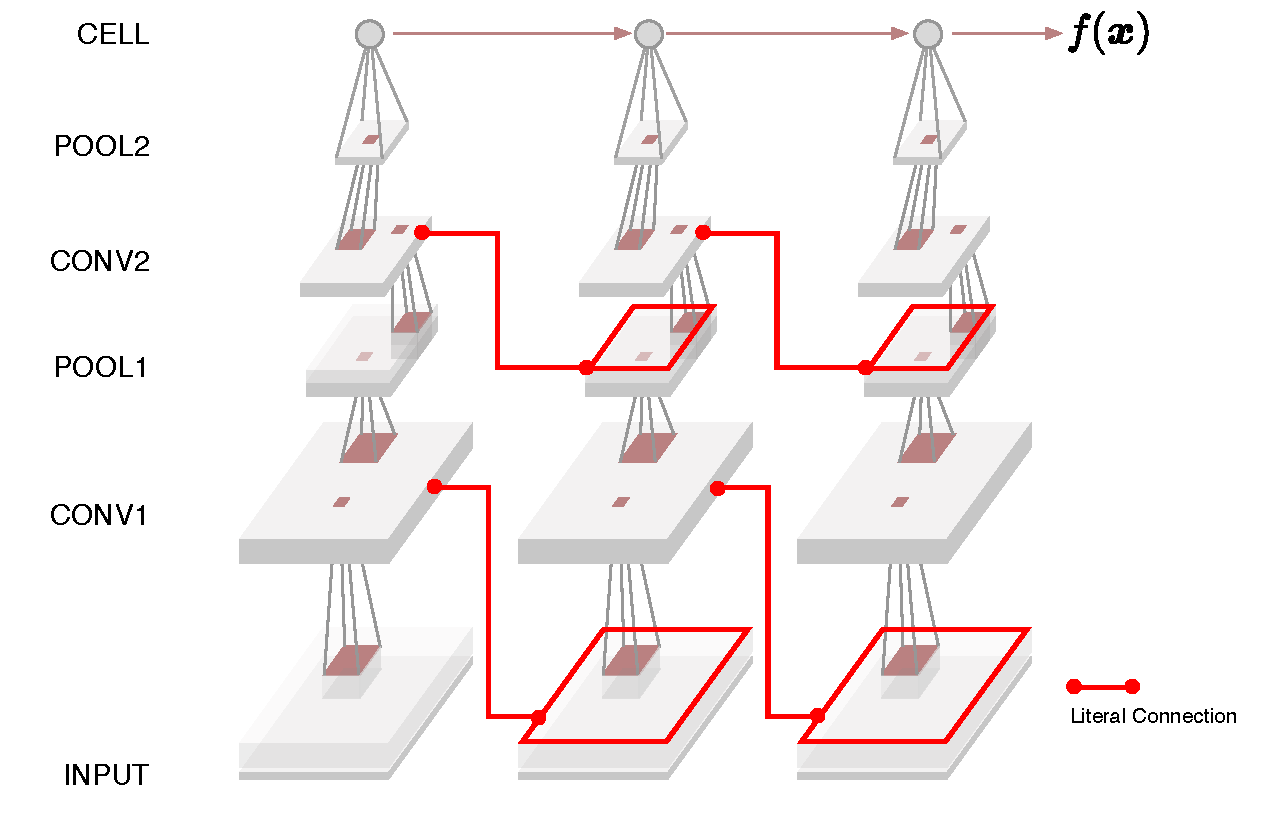
\includegraphics[width=\textwidth]{sketch/conv_literalconn}
\patcaption{ConvDeep with literal connections}{(\rnncell{Conv$^+$Deep}).} 
\label{fig:conv_literalconn}
\end{figure}

Therefore, we propose to also share results from convolution operators to the operators in the next step. We name this connections as \textit{literal connections} and \addfigure{\ref{fig:conv_literalconn}} illustrates such connections in red. From the following, we are going to refer Conv$^+$ to the setting where convolutional layers are connected through the literal connections. 

%\subsection{Setting}
In this experiment, we divided results into 2 parts. The first part focuses on stationary dropout and R-LSTM proposal and use the Deep architecture as a baseline. We refer models trained with stationary dropout with $-SD$ suffix. For R-LSTM's configuration, we also added one layer with 256 neurons between the input and 75 R-LSTM cells to make it comparable to the Deep architecture.  \todo{Figure X : show R-LSTM setting}

In the second part, we are going to discuss results from the literal connection proposal as well as results from ConvR-LSTM where the first fully-connected layer is replaced by convolutions and pooling layers with the same configuration as in ConvDeep. The number of R-LSTM cells is also the same to the first part. 

\todo{figure describe R-LSTM settings with cell?}


\subsection{Result}
Table \ref{tab:maj_exp3_model_acc} shows number of trainable parameters in the proposed architectures as well as accuracy.

\renewcommand{\arraystretch}{1.5}
\begin{table}[h]
\begin{center}
\begin{tabular}{lc|c|c|}
\cline{3-4}
& &
\multicolumn{2}{c|}{\parbox{3.5cm}{ \vskip 1mm \centering \textbf{Accuracy} \vskip 1mm}} \\ \hline
\multicolumn{1}{|l|}{\textbf{Cell architecture}} & \textbf{No. variables} & \textbf{MNIST-MAJ} & \textbf{FashionMNIST-MAJ} \\ \hline
\multicolumn{1}{|l|}{Deep-SD}                  & 153,578             & 98.10\% & 89.47\% \\ 
\multicolumn{1}{|l|}{R-LSTM}                    & 145,701   & 98.50\% & 91.35\% \\ 
\multicolumn{1}{|l|}{R-LSTM-SD}              &  145,701                & 98.57\% & 91.52\% \\ 
 \multicolumn{1}{|l|}{Conv$^+$Deep}       & 175,418                 & 97.92\% & 88.10\% \\
 \multicolumn{1}{|l|}{ConvR-LSTM-SD}      & 152,125                 & 99.35\% & 93.60\%  \\ 
\multicolumn{1}{|l|}{Conv$^+$R-LSTM-SD}   & 175,741                & 98.48\% & 88.19	\%  \\ \hline 
\end{tabular}

\end{center}
\caption{Number of trainable variables and model accuracy of the  proposed architectures for MNIST-MAJ and FashionMNIST-MAJ.}
\label{tab:maj_exp3_model_acc}
\end{table}
\renewcommand{\arraystretch}{1}


\subsubsection{Stationary Dropout and R-LSTM}
 \begin{figure}[!htb]
\centering
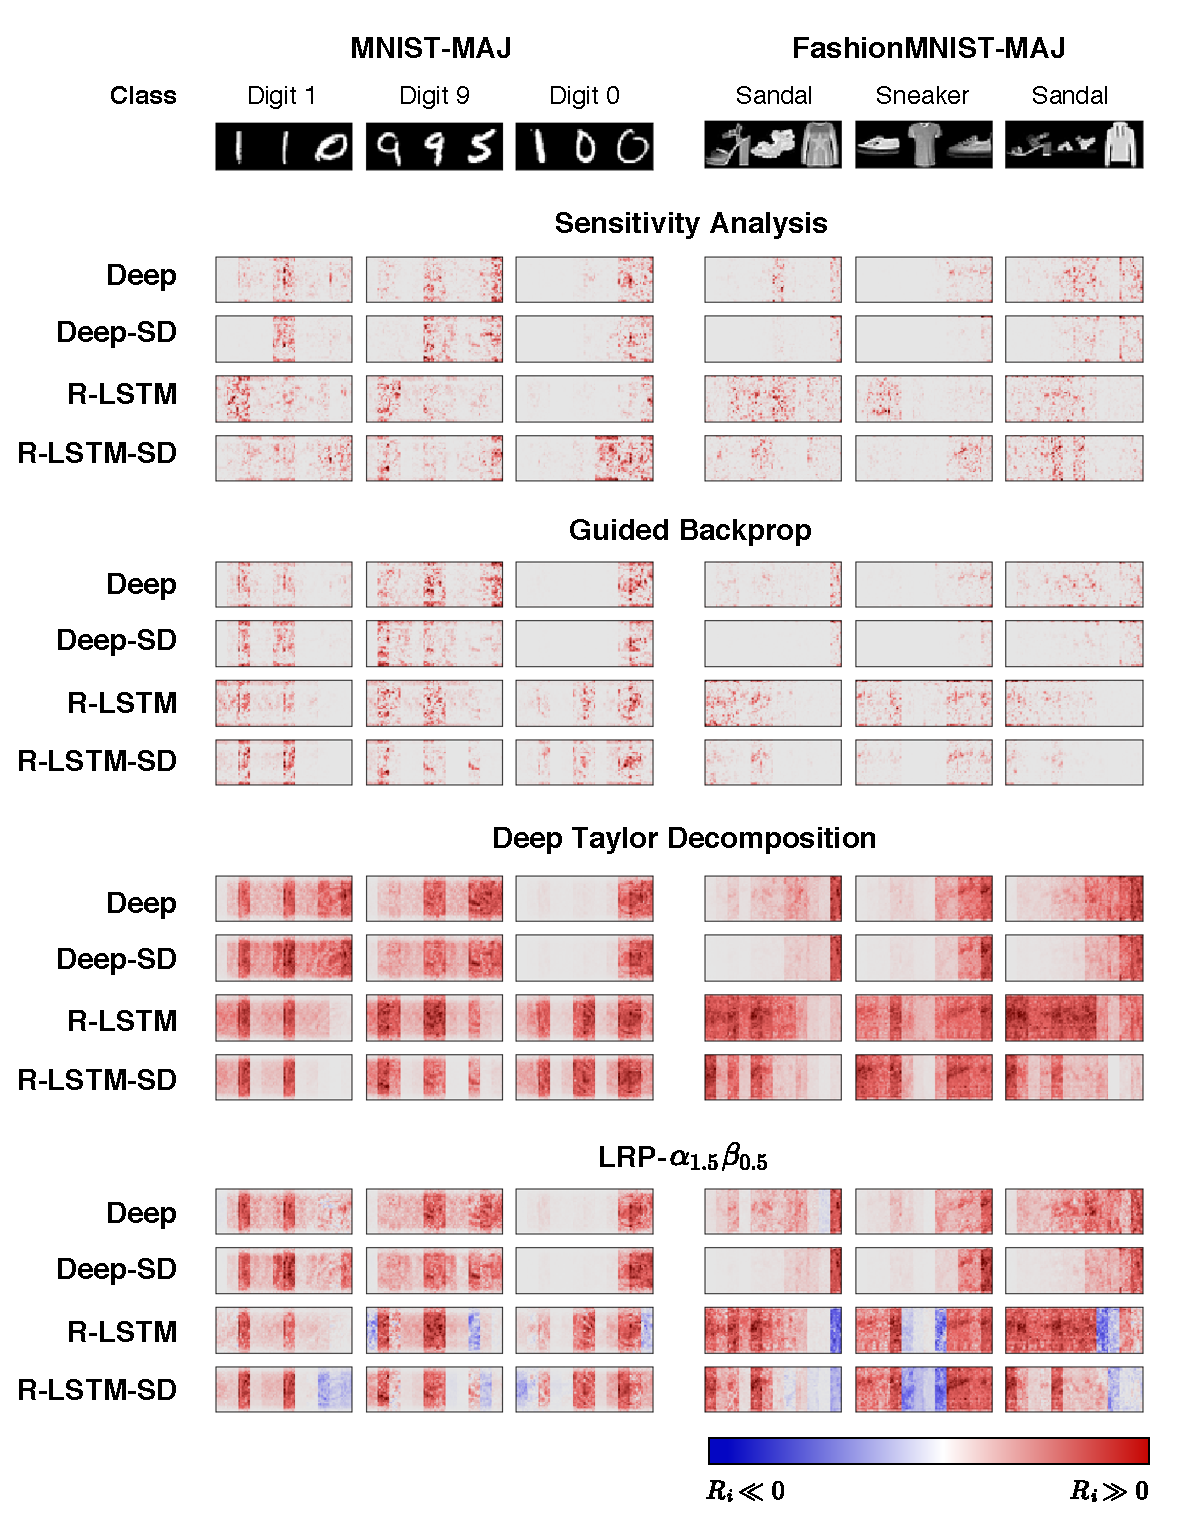
\includegraphics[width=\textwidth]{sketch/heatmap_msc_rlstm_exp}
\patcaption{Relevance heatmaps produced by different explanation techniques on Deep and R-LSTM architecture trained on MNIST-MAJ and FashionMNIST-MAJ with sequence length $T=12$ and different dropout configurations.}{\heatmapscaleexplain} 
\label{fig:heatmap_msc_rlstm_exp}
\end{figure}

\addfigure{\ref{fig:heatmap_msc_rlstm_exp}} shows results of the first part of this experiment. Here, variants of Deep and R-LSTM are compared. From the figure, it is obvious that R-LSTM provides better explanations than the Deep architecture. More precisely, we can directly observe the improvements from GB, DTD and $\lrpp$ heatmaps. Moreover, training with stationary dropout seems to produce R-LSTM with higher explanation capability. This is well notable on explanations from  DTD and $\lrpp$. In contrast, stationary dropout does not seem to have any prominent impact on the Deep architecture.


 \begin{figure}[!htb]
\centering
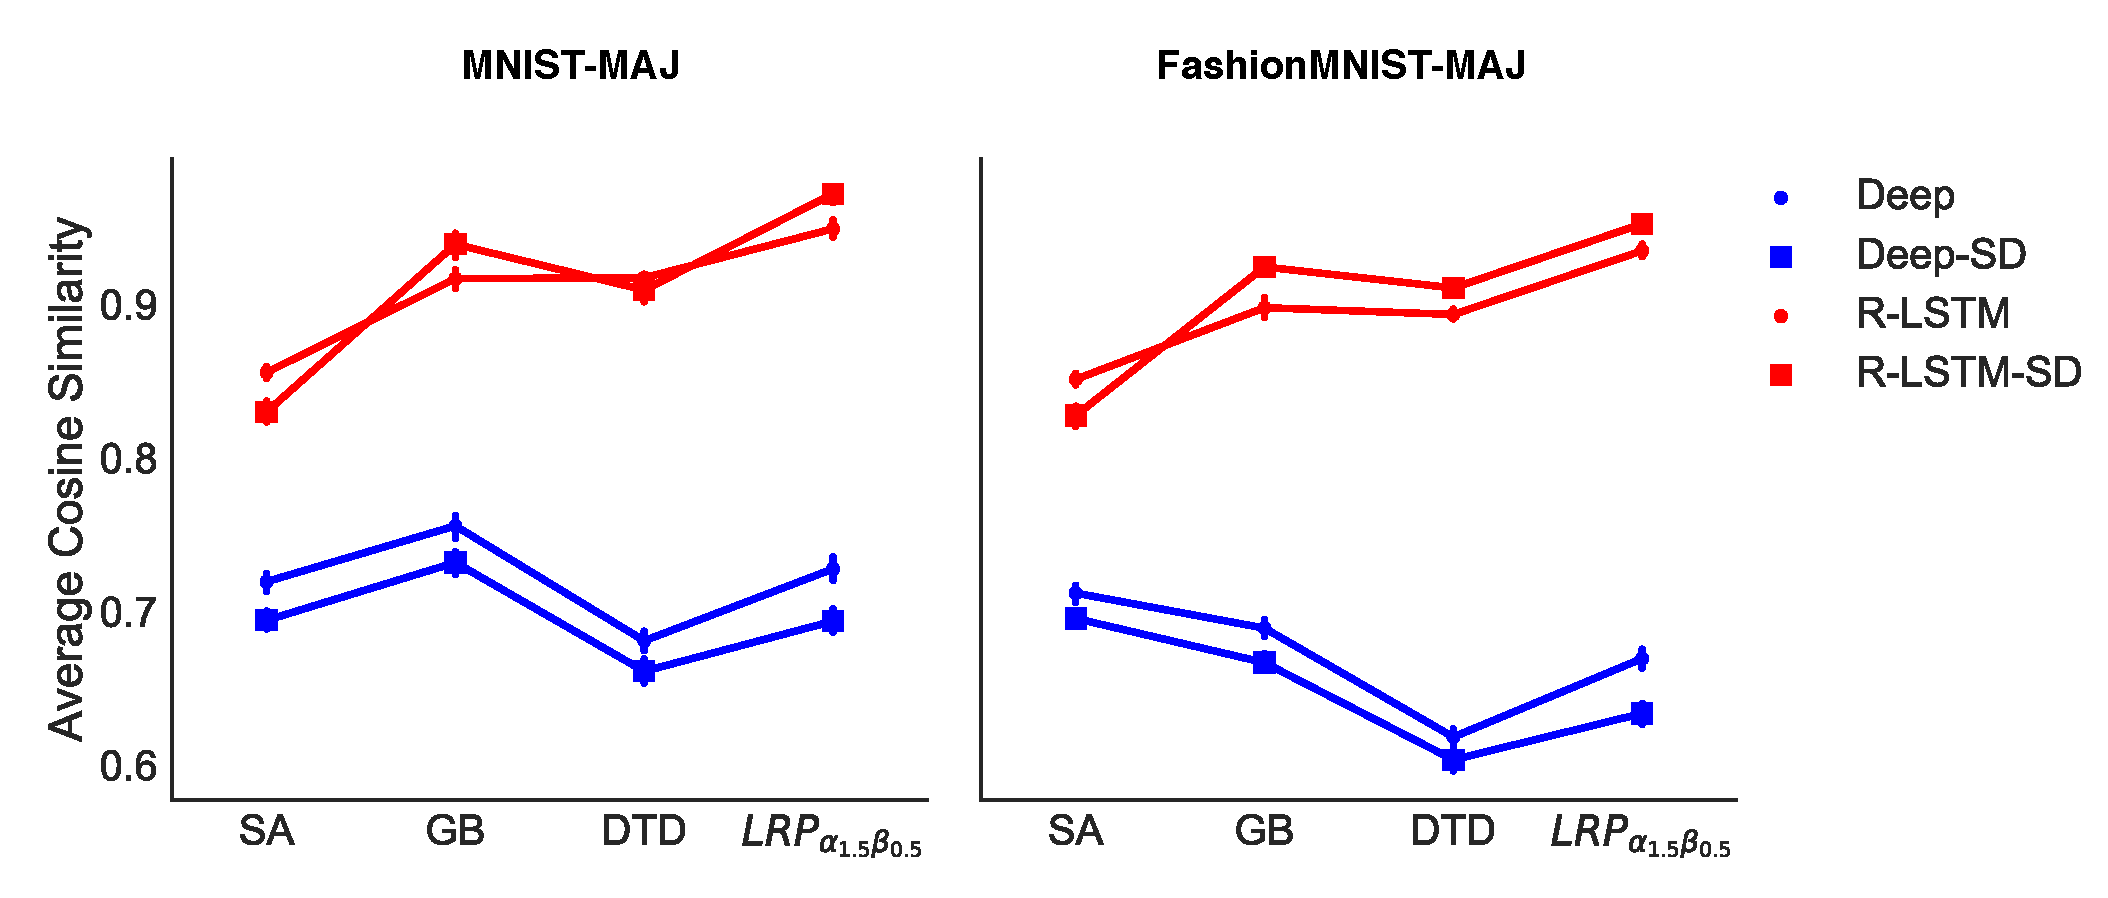
\includegraphics[width=\textwidth]{sketch/rel_dist_rlstm_exp}
%\caption{}  }. 
\patcaption{Average cosine similarity from different explanation techniques and Deep and R-LSTM architecture.}{The values are averaged from cross-validation results and the vertical lines depicted 95\% confidence interval. The baseline is the Deep architecture depicted by dotted blue line. Accuracy of the models can be found at Appendix  \ref{annex:model_acc}}

\label{fig:rel_dist_rlstm_exp}
\end{figure}

\addfigure{\ref{fig:rel_dist_rlstm_exp}} presents the quantitative evaluation. As a reminder, these plots are cosine similarity averaged over models trained with cross validation procedure described in  Section \ref{sec:evaluation_med}. The figure shows that R-LSTM significantly improves relevance distribution than the Deep architecture regardless of explanation techniques.  This means that R-LSTM is more explainable than the Deep architecture. Similar to one observation in Section \ref{sec:exp1_result}, we also see that the proportion of the improvement of DTD and LRP seem to have greater advantage from R-LSTM than the other methods.  

\addfigure{\ref{fig:rel_dist_rlstm_exp}}  also shows another interesting result. We can see that R-LSTM trained with stationary dropout, or R-LSTM-SD, produces better explanations than R-LSTM on FashionMNIST-MAJ, although the difference does not obvious on MNIST-MAJ. This might be due to complexity of FashionMNIST samples' structures, as a result keeping dropout mask the same for all step would enable the network to efficiently learn latent features from homogenous input. In contrast, this does not seem to be the case for the Deep architecture. Particularly, we find that the cosine similarity measurement of Deep-SD is lower than Deep in any case.

\todo{hypo thesis?}
\clearpage

\subsubsection{ConvDeep with literal connections and ConvR-LSTM}
 \begin{figure}[!htb]
\centering
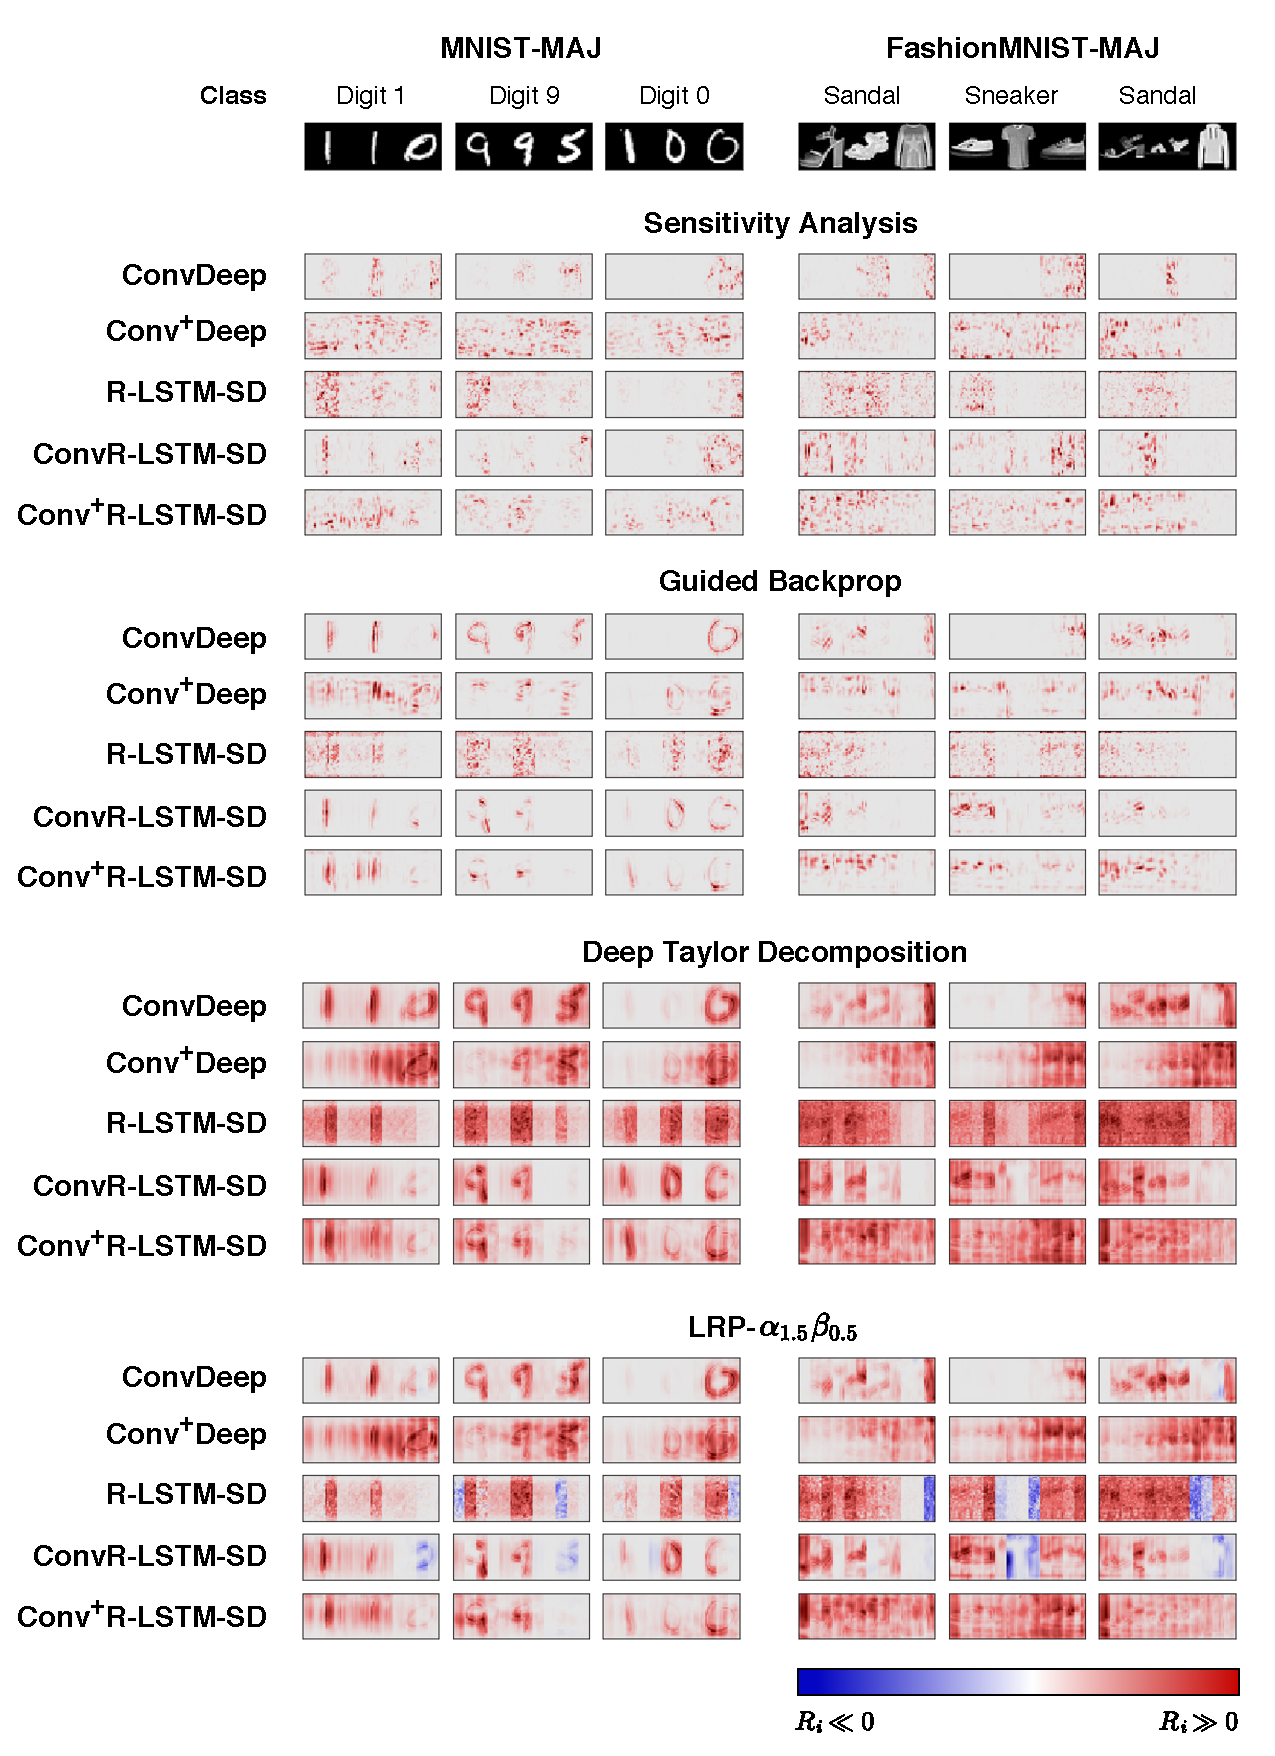
\includegraphics[width=\textwidth]{sketch/heatmap_msc_convtran_exp_v2}
\patcaption{Relevance heatmaps produced by different explanation techniques on variants of ConvDeep and R-LSTM architecture trained on MNIST-MAJ and FashionMNIST-MAJ with sequence length $T=12$.}{\heatmapscaleexplain} 
\label{fig:heatmap_msc_convtran_exp}
\end{figure}
For the second part, we compare the ConvDeep architecture and the effect of literal connections as well as R-LSTM-SD with convolutional layers, which is referred as ConvR-LSTM-SD. According to \addfigure{\ref{fig:heatmap_msc_convtran_exp}}, Conv$^+$Deep produces more diffuse relevance heatmaps than ConvDeep. This is specially notable on heatmaps from SA  and GB method. Similarly, Conv$^+$Deep also produces worse results for DTD and $\lrpp$, for example consider Digit 1 and Digit 9 sample, where the relevance scores are unnecessarily distributed to the last digit's block. 

\addfigure{\ref{fig:heatmap_msc_convtran_exp}} also shows relevance heatmaps from ConvR-LSTM-SD whose first fully-connected layer is replaced by 2 convolutional and pooling layers. Comparing to R-LSTM-SD, having convolutional and pooling layers does improve  the quality of the heatmaps further. In particular, we can clearly see samples' structures from the explanations. \addfigure{\ref{fig:heatmap_msc_convrlstm_pos_rel}} further emphasizes the improvement introduced by the convolutional and pooling layers. Here, we plots the relevance heatmaps by using only positive relevance. We can see that the heatmaps from ConvR-LSTM-SD are proper highlighted and provide substantial  features of the samples.

 \begin{figure}[!htb]
\centering
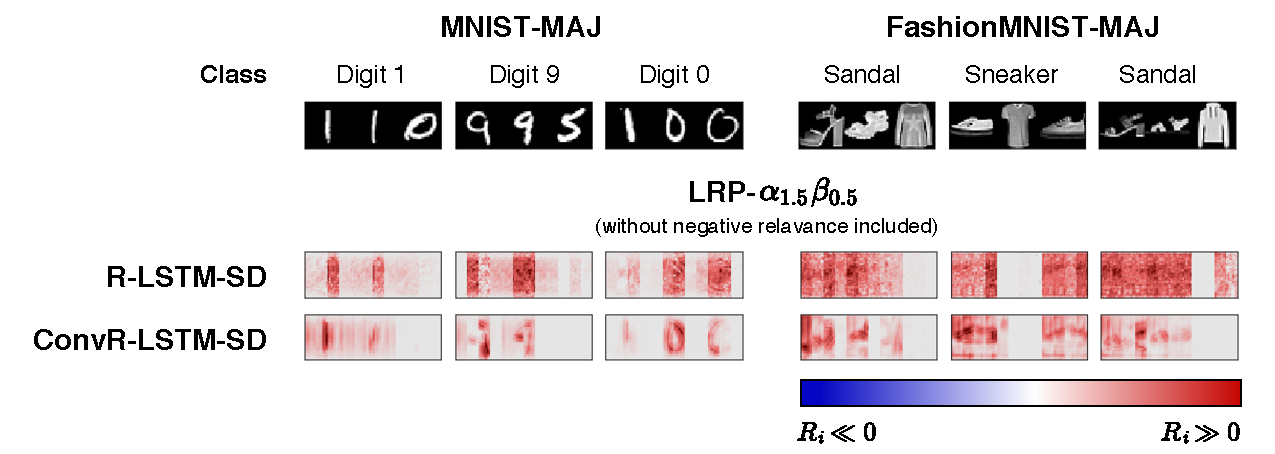
\includegraphics[width=\textwidth]{sketch/heatmap_msc_convrlstm_pos_rel}
\patcaption{Positive relevance heatmaps produced by $\lrpp$ technique on R-LSTM and ConvR-LSTM architecture trained on MNIST-MAJ and FashionMNIST-MAJ with sequence length $T=12$.}{\heatmapscaleexplain} 
\label{fig:heatmap_msc_convrlstm_pos_rel}
\end{figure}

 \begin{figure}[!htb]
\centering
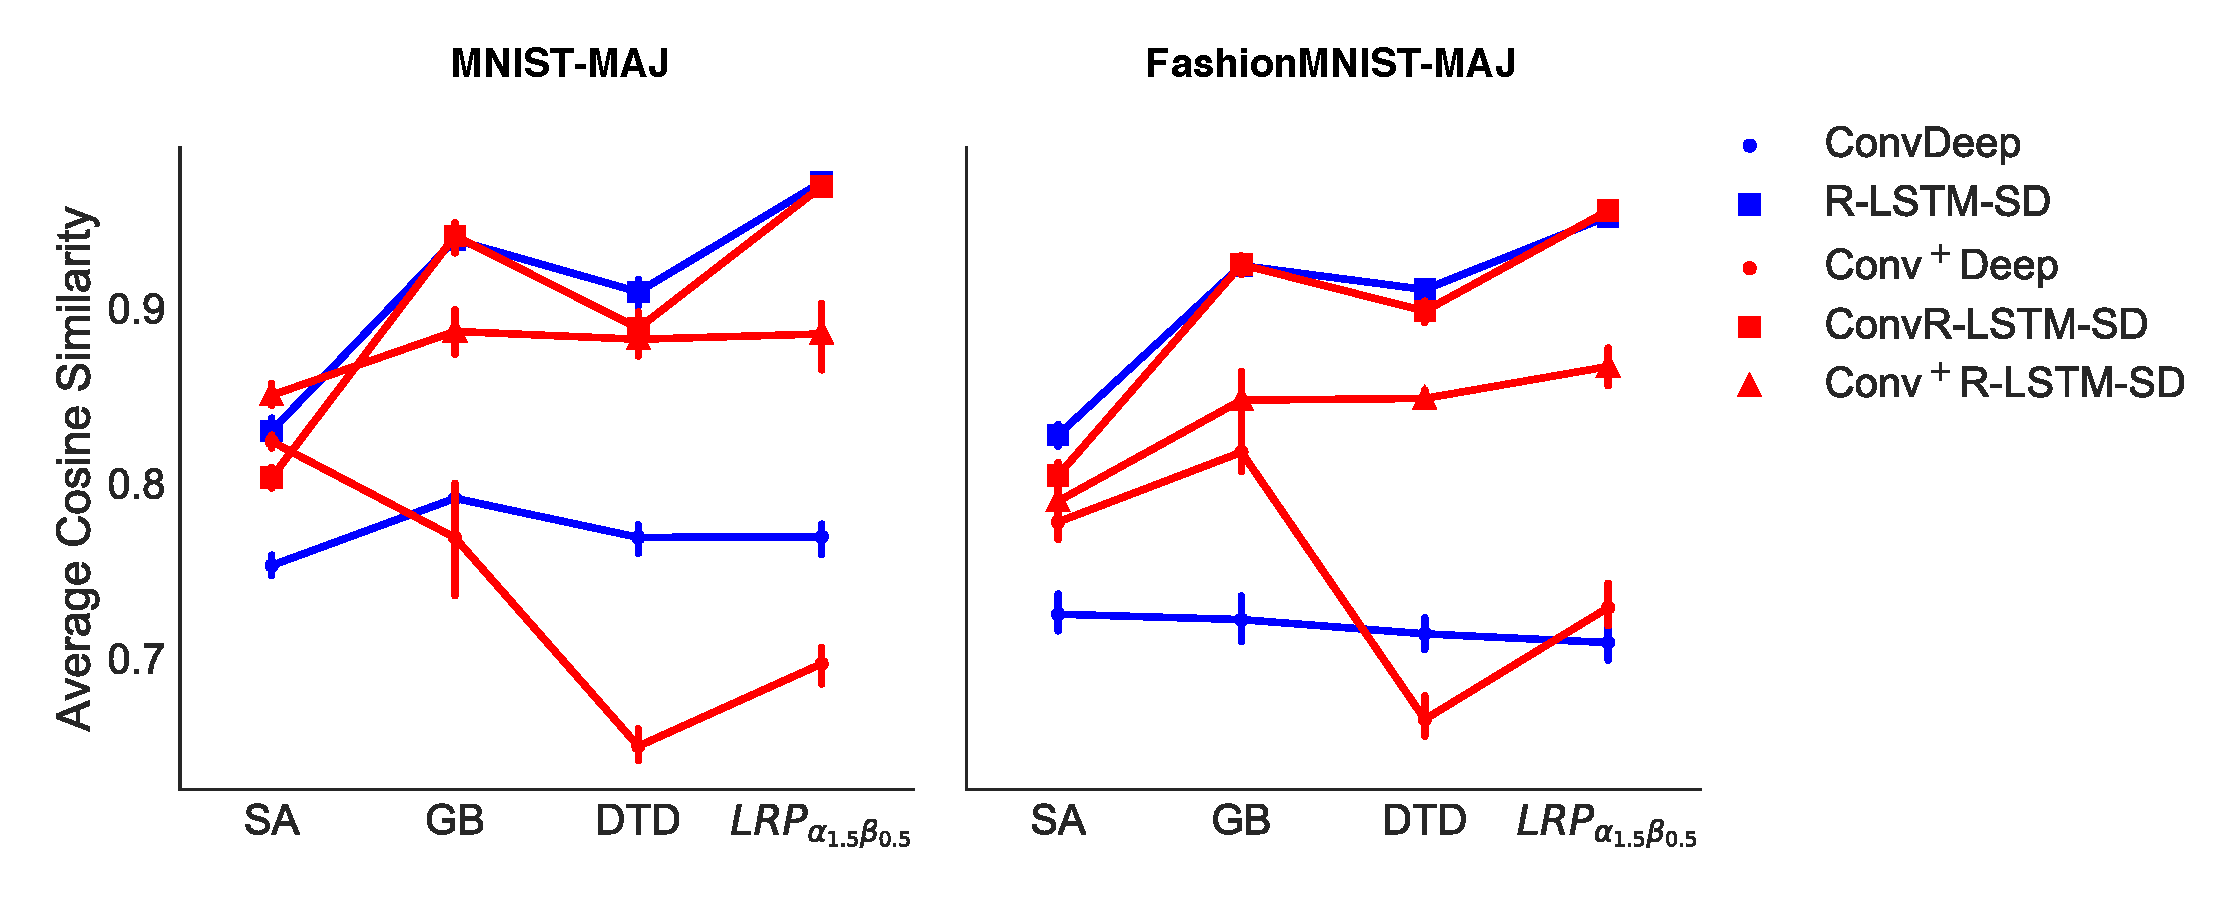
\includegraphics[width=\textwidth]{sketch/rel_dist_convdeep_trans_exp}
\patcaption{Average cosine similarity from different explanation techniques and variants of ConvDeep and R-LSTM architecture.}{The values are averaged from cross-validation results and the vertical lines depicted 95\% confidence interval. The baseline are the Deep and R-LSTM-SD architecture represented in blue. Accuracy of the models can be found at Appendix \ref{annex:model_acc}} 
\label{fig:rel_dist_convdeep_trans_exp}
\end{figure}

\addfigure{\ref{fig:rel_dist_convdeep_trans_exp}} presents the cosine similarity measurement this second part of the experiment. Here, ConvDeep and R-LSTM-SD are results from the previous experiments and used as baseline. Unexpectedly, having literal connections in ConvDeep does not seem to show consistent influence between MNIST-MAJ and FashionMNIST-MAJ. However, the connections considerably reduce the explanation capability of the ConvR-LSTM-SD architecture. 
 Although explanations from ConvR-LSTM-SD are less noisy and contain impressive structures from the input as shown in \addfigure{\ref{fig:heatmap_msc_convrlstm_pos_rel}}, the average cosine similarity of R-LSTM-SD and ConvR-LSTM-SD look almost identical. This is due to the fact our cosine similarity measurement operates on scalar values but not structures inside explanation heatmaps.
 
 \todo{hypo: In fact, using Tukey HSD test shows that the improvement is not statistically significant} 
\todo{hypothesis testing}

\clearpage

\subsection{Summary}
Results from this experiment shows some successful improvements from what we have seen on Sectoin \ref{sec:exp2}. In particular, employing gating unit and keeping dropout activities the same significantly improve explanation ability of RNN models on any explanation method.  

Moreover, convolutional and pooling layers enables the models to produce explanations with more perceivable input features than traditional fully-connected layers, although this improvement does not seem to be well captured by cosine similarity that we proposed to use. . This illustrates  a shortcoming of cosine similarity that we proposed to use for the quantitative evaluation.

On the other hand, literal connections do not show any consistent improvement for the settings we are considering. In fact, having wider confidence interval suggests that they seem to make explanations less stable.
